\documentclass[tikz,border=10pt]{standalone}
\usepackage{amsmath,amssymb}
\usetikzlibrary{arrows.meta,positioning,calc,decorations.pathmorphing}

\newcommand{\ord}{\operatorname{ord}}

\begin{document}
	
	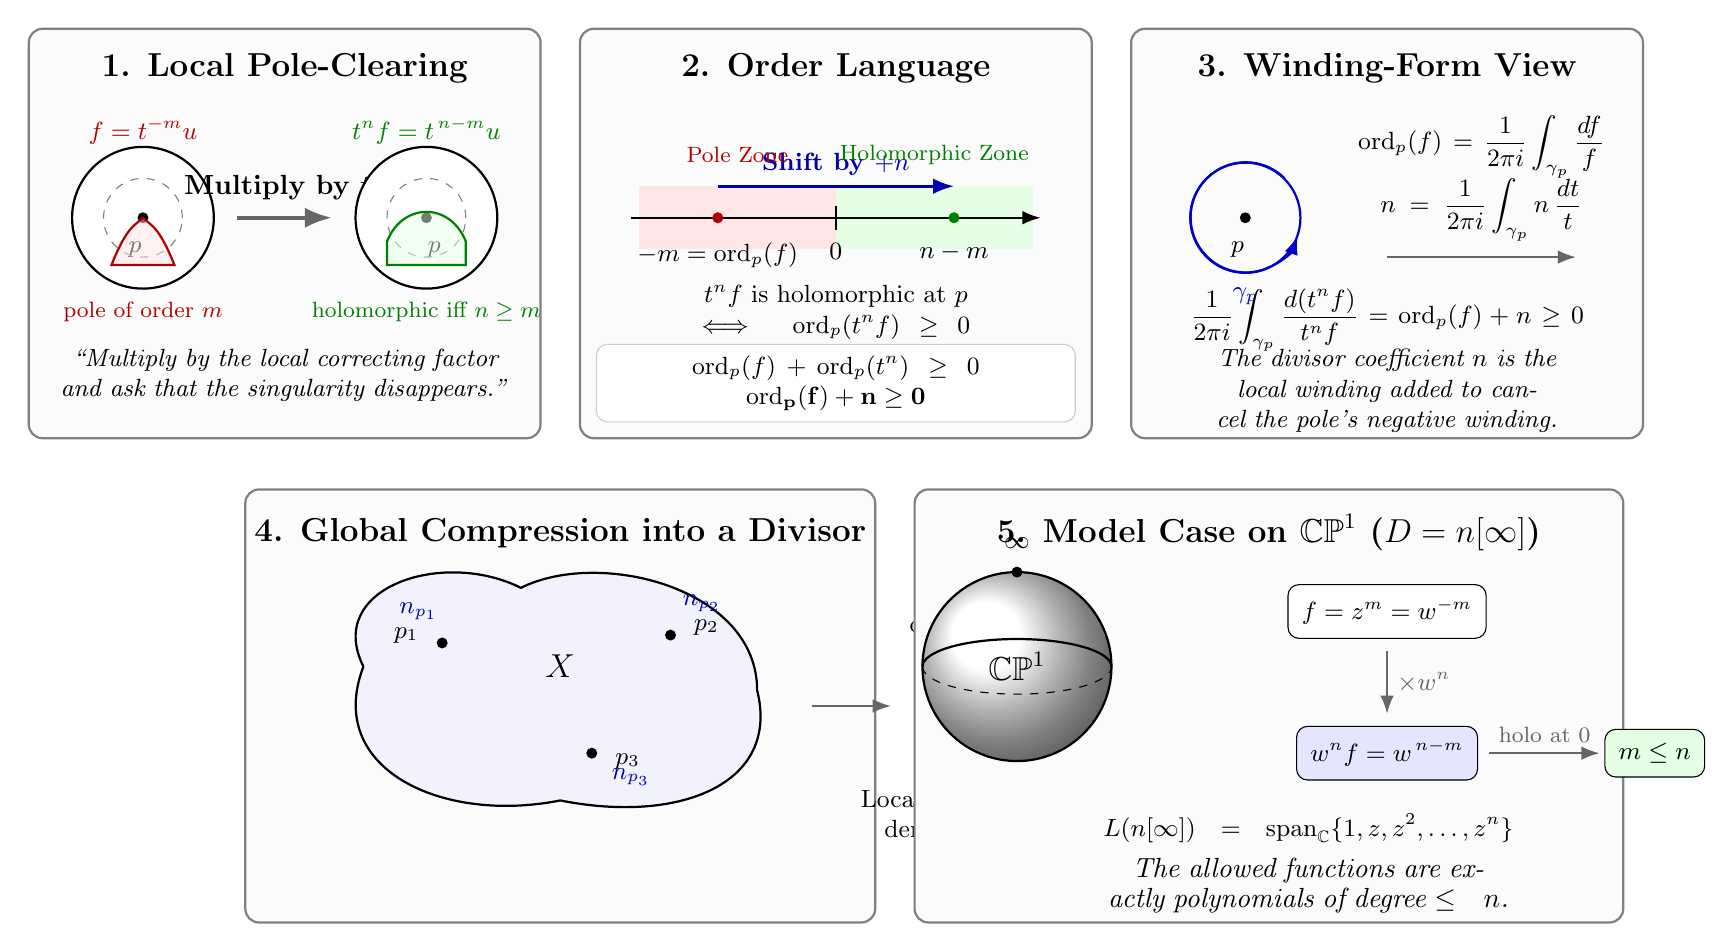
\begin{tikzpicture}[
		>=Latex,
		font=\small,
		panel/.style={draw=black!50, rounded corners=5pt, thick, fill=gray!3},
		title/.style={font=\large\bfseries},
		point/.style={circle, fill=black, inner sep=1.4pt},
		good/.style={green!50!black, thick},
		bad/.style={red!70!black, thick},
		flow/.style={->, thick, black!60},
		every node/.style={align=center}
		]
		
		% =========================================================
		% PANEL A: Local Correction (Sections 1 & 8)
		% =========================================================
		\begin{scope}[shift={(0, 4.5)}]
			\node[panel, minimum width=6.5cm, minimum height=5.2cm] (A) at (0,0) {};
			\node[title] at (0, 2.1) {1. Local Pole-Clearing};
			
			% Left local disk (Uncorrected)
			\draw[thick, fill=white] (-1.8, 0.2) circle (0.9);
			\node[point,label={[xshift=-1mm,yshift=-1mm]below:$p$}] at (-1.8, 0.2) {};
			\draw[dashed, black!50] (-1.8, 0.2) circle (0.5);
			\node[bad] at (-1.8, 1.3) {$f=t^{-m}u$};
			\node[bad, font=\footnotesize] at (-1.8, -1.0) {pole of order $m$};
			
			% "Blow-up" graphic
			\draw[bad, fill=red!10, fill opacity=0.5] (-2.2, -0.4) .. controls (-2.0, 0.1) and (-1.9, 0.1) .. (-1.8, 0.2) .. controls (-1.7, 0.1) and (-1.6, 0.1) .. (-1.4, -0.4) -- cycle;
			
			% Arrow
			\draw[flow, line width=1.5pt] (-0.6, 0.2) -- (0.6, 0.2);
			\node[above, font=\bfseries] at (0, 0.3) {Multiply by $t^n$};
			
			% Right local disk (Corrected)
			\draw[thick, fill=white] (1.8, 0.2) circle (0.9);
			\node[point,label={[xshift=1mm,yshift=-1mm]below:$p$}] at (1.8, 0.2) {};
			\draw[dashed, black!50] (1.8, 0.2) circle (0.5);
			\node[good] at (1.8, 1.3) {$t^n f=t^{\,n-m}u$};
			
			% Smooth graphic
			\draw[good, fill=green!10, fill opacity=0.5] (1.3, -0.1) .. controls (1.5, 0.4) and (2.1, 0.4) .. (2.3, -0.1) -- (2.3, -0.4) -- (1.3, -0.4) -- cycle;
			\node[good, font=\footnotesize] at (1.8, -1.0) {holomorphic iff $n \ge m$};
			
			\node[text width=6cm] at (0,-1.8) 
			{\textit{``Multiply by the local correcting factor and ask that the singularity disappears.''}};
		\end{scope}
		
		% =========================================================
		% PANEL B: Order Language (Section 2)
		% =========================================================
		\begin{scope}[shift={(7, 4.5)}]
			\node[panel, minimum width=6.5cm, minimum height=5.2cm] (B) at (0,0) {};
			\node[title] at (0, 2.1) {2. Order Language};
			
			% Shaded regions on number line
			\fill[red!10] (-2.5, -0.2) rectangle (0, 0.6);
			\fill[green!10] (0, -0.2) rectangle (2.5, 0.6);
			
			% Axis
			\draw[thick,->] (-2.6, 0.2) -- (2.6, 0.2);
			\draw[thick] (0, 0.05) -- (0, 0.35);
			\node[below] at (0, 0) {$0$};
			\node[below] at (-1.5, 0) {$-m=\ord_p(f)$};
			\node[below] at (1.5, 0) {$n-m$};
			
			% Points and shift arrow
			\fill[bad] (-1.5, 0.2) circle (2pt);
			\fill[good] (1.5, 0.2) circle (2pt);
			\draw[flow, blue!70!black, line width=1pt] (-1.5, 0.6) -- node[above] {\textbf{Shift by $+n$}} (1.5, 0.6);
			
			\node[bad, font=\footnotesize] at (-1.25, 1.0) {Pole Zone};
			\node[good, font=\footnotesize] at (1.25, 1.0) {Holomorphic Zone};
			
			\node[text width=5.5cm] at (0,-1.0) 
			{$t^n f$ is holomorphic at $p$\\ $\Longleftrightarrow \quad \ord_p(t^n f)\ge 0$};
			
			\node[text width=5.8cm, fill=white, draw=black!20, rounded corners, inner sep=4pt] at (0,-1.9) 
			{$\ord_p(f) + \ord_p(t^n) \ge 0$\\ $\mathbf{\ord_p(f)+n\ge 0}$};
		\end{scope}
		
		% =========================================================
		% PANEL C: Winding Form (Section 5)
		% =========================================================
		\begin{scope}[shift={(14, 4.5)}]
			\node[panel, minimum width=6.5cm, minimum height=5.2cm] (C) at (0,0) {};
			\node[title] at (0, 2.1) {3. Winding-Form View};
			
			% Loop and point
			\node[point,label={[xshift=-1mm,yshift=-1mm]below:$p$}] at (-1.8, 0.2) {};
			\draw[thick, blue!80!black] (-1.8, 0.2) circle (0.7);
			\draw[->, thick, blue!80!black] (-1.3, 0.7) arc[start angle=45,end angle=340,radius=0.7];
			\node[blue!80!black] at (-1.8, -0.8) {$\gamma_p$};
			
			% Formulas
			\node[text width=3.8cm] at (1.2, 1.1) 
			{$\displaystyle \ord_p(f)=\frac{1}{2\pi i}\int_{\gamma_p}\frac{df}{f}$};
			
			\node[text width=3.8cm] at (1.2, 0.3) 
			{$\displaystyle n = \frac{1}{2\pi i}\int_{\gamma_p} n\,\frac{dt}{t}$};
			
			\draw[flow] (0, -0.3) -- (2.4, -0.3);
			
			\node[text width=5.5cm] at (0, -1.1) 
			{$\displaystyle \frac{1}{2\pi i}\int_{\gamma_p}\frac{d(t^n f)}{t^n f} = \ord_p(f)+n\ge 0$};
			
			\node[text width=6cm] at (0, -2.0) 
			{\textit{The divisor coefficient $n$ is the local winding added to cancel the pole's negative winding.}};
		\end{scope}
		
		% =========================================================
		% PANEL D: Global Compression (Sections 3 & 4)
		% =========================================================
		\begin{scope}[shift={(3.5, -1.5)}]
			\node[panel, minimum width=8cm, minimum height=5.5cm] (D) at (0,0) {};
			\node[title] at (0, 2.2) {4. Global Compression into a Divisor};
			
			% Compact surface blob
			\draw[thick, fill=blue!5] 
			(-2.5,0.5) .. controls (-3.0,1.5) and (-1.5,2.0) .. (-0.5,1.5)
			.. controls (0.5,2.0) and (2.5,1.5) .. (2.5,0.2)
			.. controls (2.8,-1.0) and (1.5,-1.5) .. (0,-1.2)
			.. controls (-1.5,-1.5) and (-3.0,-0.8) .. (-2.5,0.5);
			\node[font=\large] at (0, 0.5) {$X$};
			
			% Marked points
			\node[point,label={[xshift=-1mm,yshift=1mm]left:$p_1$}] at (-1.5, 0.8) {};
			\node[point,label={[xshift=1mm,yshift=1mm]right:$p_2$}] at (1.4, 0.9) {};
			\node[point,label={[xshift=1mm,yshift=-1mm]right:$p_3$}] at (0.4, -0.6) {};
			
			\node[blue!70!black] at (-1.8, 1.2) {$n_{p_1}$};
			\node[blue!70!black] at (1.8, 1.3) {$n_{p_2}$};
			\node[blue!70!black] at (0.9, -0.9) {$n_{p_3}$};
			
			\draw[flow] (3.2, 0) -- (4.2, 0);
			
			\node[text width=6cm] at (6.5, 1.2) 
			{\textbf{Global Condition:}\\ $\ord_p(f)+n_p\ge 0$ for \emph{all} $p$.};
			
			\node[draw, rounded corners=4pt, fill=blue!10, inner sep=6pt, font=\large] at (6.5, 0) 
			{$\operatorname{div}(f)+D\ge 0$};
			
			\node[text width=6.5cm] at (6.5, -1.2) 
			{\textbf{Vector Space $L(D)$}\\ Local holomorphicity is preserved under sums, forming a vector space.};
		\end{scope}
		
		% =========================================================
		% PANEL E: CP^1 Model Case (Section 7)
		% =========================================================
		\begin{scope}[shift={(12.5, -1.5)}]
			\node[panel, minimum width=9cm, minimum height=5.5cm] (E) at (0,0) {};
			\node[title] at (0, 2.2) {5. Model Case on $\mathbb{CP}^1$ ($D=n[\infty]$)};
			
			% Sphere / Projective Line
			\shade[ball color=white] (-3.2, 0.5) circle (1.2);
			\draw[thick] (-3.2, 0.5) circle (1.2);
			\draw[dashed] (-4.4, 0.5) arc[start angle=180,end angle=360,x radius=1.2,y radius=0.35];
			\draw[thick] (-2.0, 0.5) arc[start angle=0,end angle=180,x radius=1.2,y radius=0.35];
			\node[font=\large] at (-3.2, 0.5) {$\mathbb{CP}^1$};
			\node[point,label={[yshift=1mm]above:$\infty$}] at (-3.2, 1.7) {};
			
			% Monomial Transformation
			\node[draw, rounded corners=4pt, fill=white, inner sep=5pt] at (1.5, 1.2) {$f=z^m=w^{-m}$};
			
			\draw[flow] (1.5, 0.7) -- node[right] {$\times w^n$} (1.5, -0.1);
			
			\node[draw, rounded corners=4pt, fill=blue!10, inner sep=5pt] at (1.5, -0.6) {$w^n f=w^{\,n-m}$};
			
			\draw[flow] (2.8, -0.6) -- node[above, font=\footnotesize] {holo at 0} (4.2, -0.6);
			
			\node[draw, rounded corners=4pt, fill=green!10, inner sep=5pt] at (4.9, -0.6) {$m\le n$};
			
			\node[text width=8.5cm, align=center] at (0.5, -2.0) 
			{$\displaystyle L(n[\infty]) = \operatorname{span}_{\mathbb{C}}\{1,z,z^2,\dots,z^n\}$\\[1ex]
				\normalsize \textit{The allowed functions are exactly polynomials of degree $\le n$.}};
		\end{scope}
		
	\end{tikzpicture}
	
\end{document}